\maketitle

\begin{abstract}
Simple Linux Utility for Resource Management (SLURM) is an open source,
fault-tolerant, and highly scalable cluster management and job 
scheduling system for Linux clusters of 
thousands of nodes.  Components include machine status, partition
management, job management, and scheduling modules.  The design also 
includes a scalable, general-purpose communication infrastructure.
Development will take place in four phases:  Phase I results in a solid
infrastructure;  Phase II produces a functional but limited interactive 
job initiation capability without use of the interconnect/switch; 
Phase III provides switch support and documentation; Phase IV provides 
job statusing, fault-tolerance, and job queueing and control through  
Livermore's Distributed Production Control System (DPCS), a metabatch and
resource management system.
\end{abstract}

\vspace{0.25in}

%\begin{center}
%
\epsfig{file=slurm.eps,width=4in}
%\end{center}

\newpage



\section{Overview}

SLURM\footnote{A tip of the hat to Matt Groening and creators of {\em Futurama},
where Slurm is the highly addictive soda-like beverage made from worm
excrement.} (Simple Linux Utility for Resource Management) 
is a resource managment 
system suitable for use on Linux clusters, large and small.  After surveying 
resource managers available for Linux (see Appendix~\ref{survey}) and finding 
none that were simple, highly scalable, and portable to different cluster 
architectures and interconnects, the authors set out to design a new system.

The result is a resource management system with the following general
characteristics:

\begin{itemize}
\item {\em Simplicity}: SLURM is simple enough to allow motivated end users
to understand its source code and add functionality.  The authors will 
avoid the temptation to add features unless they are of general appeal.

\item {\em Open Source}: SLURM is available to everyone and will remain free;
its source code is distributed under the GNU General Public License.

\item {\em Portability}: SLURM is written in the C language, with a GNU 
autoconf configuration engine.  While initially written for Linux, 
other UNIX-like operating systems should be easy porting targets.

\item {\em Interconnect independence}: Initially, SLURM supports TCP/IP based
communication and the Quadrics Elan3 interconnect.  Adding support for other
interconnects is straightforward.  Users select the supported interconnects
at compile time via GNU autoconf.

\item {\em Scalability}: SLURM is designed for scalability to a 
{\em ludicrious}\footnote{The authors define a {\em ludicrious} 
number of nodes to be $2^{16} = 65536$.} number of nodes.

\item {\em Fault tolerence}: SLURM can handle a variety of failure modes
without terminating workloads, including crashes of the node running the SLURM
controller.

\item {\em Secure}: SLURM employs crypto technology to authenticate 
users to services and services to services.  
A Kerberos V / DCE infrastructure can be utillized if available.
SLURM does not assume that its networks are physically secure.

\item {\em System administrator friendly}: SLURM is configured with a few
simple configuration files and minimizes distributed state.  Its interfaces
are scriptable and its behavior is highly deterministic.

\end{itemize}

\subsection{What is SLURM?}

As a cluster resource manager, SLURM has three key functions.  First,
it allocates exclusive access to resources (compute nodes) to users for 
some duration of time so they can perform work.  Second, it provides 
a framework for starting up, executing, and monitoring work (normally a 
parallel job) on the set of allocated nodes.  Finally, it arbitrates 
conflicting requests for resources by managing batch queues.

Users interact with SLURM through three command line utilities: 
{\tt srun} for submitting a job for execution and optionally controlling it
interactively; 
{\tt scancel} for early termination of a job; 
and {\tt squeue} for monitoring queues.

System administrators perform priviledged operations through an additional
command line utility: {\tt slurmadmin}.

External schedulers and metabatch systems can submit jobs to SLURM and
order its queues through an application programming interface (API).

Compute nodes simply run a {\tt slurmd} daemon (similar to a remote shell 
daemon) to export control to SLURM.  The central controller daemon,
{\tt slurmctrld}, maintains the global state and directs operations.

\subsection{What SLURM is Not}

SLURM is not a sophisticated batch system.  Its default scheduler
implements FIFO with backfill and does not include the bells and 
whistles needed to implement complex site policy.
SLURM does however provide a sufficiently sophisticated API for an external 
scheduler or metabatch system to order its queues based on site policy.

SLURM is not a gang scheduler and does not support time sharing of compute
nodes.  SLURM clusters are space shared, and parallel jobs are always 
assigned whole nodes.  SLURM will not preempt an executing job to run a 
higher priority one (since it has no concept of priorities), but it is 
possible for an external scheduler to terminate jobs and requeue them in a 
different order via the API.

SLURM is not a metabatch system like Globus or DPCS (Distributed Production 
Control System).  SLURM supports resource management across a single cluster.

SLURM is not a comprehensive cluster administration or monitoring package.  
While SLURM knows the state of its compute nodes, it makes no attempt to put
this information to use in other ways, such as with a general purpose event
logging mechanism or a back-end database for recording historical state.
It is expected that SLURM will be deployed in a cluster along side other 
tools that perform these functions. 

\section{Architecture}

\begin{figure}
\epsfig{file=arch.eps,width=6in}
\caption{SLURM Architecture}
\label{arch}
\end{figure}

As depicted in Figure~\ref{arch}, SLURM consists of a central
{\tt slurmctrld} daemon running on a management node (with optional 
failover twin), a {\tt slurmd} daemon running on each compute node, 
and a four command line utilities: {\tt srun}, {\tt scancel}, {\tt squeue}, 
and {\tt slurmadmin}, which can run anywhere in the cluster.
A scalable communications library ties these components together.

\subsection{Controller}

\begin{figure}
\epsfig{file=LCM.arch.eps,width=6in}
\caption{SLURM Controller Architecture}
\label{controllerarch}
\end{figure}

The controller includes the following subsystems, shown in 
Figure~\ref{controllerarch}:

\begin{itemize}
\item {\em Machine and job status}: Monitor and record the state of each 
node in the cluster.

\item {\em Partition management}: Distinct functionality or capabilities 
are associated with different sets of nodes in the cluster.  Each such set 
of nodes is considered a partition. 

\item {\em Job management}: Accept, initiate, delete and otherwise manage 
the state of all jobs in the system.

\item {\em Scheduling}: Decide when and where to initiate pending jobs.

\item {\em Switch management}: Perform any interconnect-related 
monitoring and control needed to run a parallel job.

\end{itemize}

Each of these subsystems is described in detail below.

\subsubsection{Machine Status}

One SLURM daemon will be required on each node in the cluster.
One module of that daemon will monitor its state.
While existing tools can be combined for machine status and management, such an
arrangement lacks the scalability required for the support of thousands of
nodes. We believe this poses serious problems in the management of large Linux
clusters and feel compelled to address this issue. 

We recognize the severe impact system daemons can have on performance of
parallel jobs, so the compute and memory resources consumed by this daemon
should be minimized. In phase three, we intend for this service to also monitor
basic job state information. In phase four, this will be expanded to include 
job accounting information. Providing all functions
within a single daemon will minimize system overhead. Node information that we
intend to monitor includes:

\begin{itemize}
\item Count of processors on the node
\item Size of real memory on the node
\item Size of temporary disk storage
\item Partition(s) serving
\item State of node (RUN, IDLE, DRAIN, etc.)
\item Cumulative CPU use (by job, kernel and daemons, possibly reporting 
both user and system time independently)
\item Allocated CPU time (recognizes preempted time, by job, kernel and daemons)
\item Real memory demand (by job, kernel and daemons)
\end{itemize}

The SLURM administrator could specify, at a minimum ,a list of system node 
names using a regular expression. 
If he requires more than one partition, that information should also be specified. 
He may also specify the mimimanl node configuration values which are acceptable 
(CPU count, real memory size, etc.). He could alternately let the individual 
nodes register their actual configurations into the database and save that 
as a baseline configuration in order to note discrepancies when nodes register 
on future SLURM initiations.

This information is readily available through system calls and reading the
process table. DPCS daemons and the commands \textit{top} and \textit{df} 
currently collect the above data are available as models for SLURM development. 
The communications protocols in those daemon and logic to associate processes 
with jobs would require modification.

The current SLURM design only supports the allocation of entire nodes to 
jobs. Our customers at LLNL have expressed the opinion that sharing of 
nodes can severely reduce their job's performance and even reliability. 
This is due to contention for shared resources such as local disk space, 
real memory, virtual memory and processor cycles. The proper support of 
shared resources, including the enforcement of limits on these resources, 
entails a substantial amount of additional effort. Given such a cost to 
benefit situation at LLNL, we have decided to not support shared nodes. 
However, we have designed SLURM so as to not preclude the addition of 
such a capability at a later time if so desired.

It is not likely that each node in the cluster could report such information
directly to the control machine without severe scalability constraints. This
could be remedied by using intermediate nodes in a hierarchical fashion to
coalesce the data. These nodes could be ones not designated for parallel job
execution (e.g. login or I/O processing nodes). A status manager will be
required on the control machine to detect and respond to anomalies as well as
maintain the records. This data collection system is similar to that
implemented in DPCS. 

\subsubsection{Partition Management}

Partition management will be used to identify groups of nodes to be used for
execution of user jobs. Data to be associated with a partition will include:
\begin{itemize}
\item ID number
\item Access permitted, under direct user (e.g. INTERACTIVE) or system (e.g. BATCH QUEUE) control
\item List of associated nodes
\item State of partition (UP or DOWN)
\end{itemize}

It will be possible to alter this data in real-time in order to effect the
scheduling of pending jobs (currently executing jobs would continue). Unlike some
other parallel job management systems, we believe this information can be
confined to the SLURM control machine for better scalability. It would be used
by the Job Manager and Machine Status Manager, which exist only on the control
machine. An API to manage the partitions would be developed first, followed by
a simple command-line tool utilizing the API.

\subsubsection{Switch Management}

A daemon on each compute node would be responsible for allocating switch
channels and assigning them to user jobs. The switch channels would be
de-allocated upon job termination. Switch health monitoring tools will 
also be implemented in phase two. It may be desirable for the SLURM daemons to use the
switch directly for communications, particularly for the movement of a large 
executable and/or standard input file. This option will be investigated in phase
three. 

\subsubsection{Job Management}

Jobs will be allocated entire nodes. Node sharing will be supported only temporally (e.g.
time-slicing or  gang scheduling). The core functions to be supported include:
\begin{itemize}
\item Initiate job\footnote{There are considerable issues regarding allocation 
of resources (nodes) to jobs and then associating the  allocation to the job 
as well as relinquishing the allocation at job termination that we need to 
discuss. - Bob Wood}
\item Will job run query (test if "Initiate job" request would succeed)
\item Status job (including node list, memory and CPU use data)
\item Signal job for termination (following DPCS model of explicit application
registration)
\item Terminate job (remove all processes)
\item Preempt/resume job 
\item Checkpoint/restart job (future)
\item Change node count of running job (could fail if insufficient resources are 
available, future)
\end{itemize}

Submitted jobs can specify desired partition, CPU count, node count, task 
count, task distribution pattern (round-robin or sequential within a node), 
and (optionally) an explicit list of nodes. The submitted job will be 
identified as being initiated under direct user (e.g. INTERACTIVE) or system 
(e.g. BATCH QUEUE) control, and by virtue of this can be constrained 
to specific partitions. 

Since scheduling decisions are being provided by the scheduling component,
there is no concept of submitting a job to be queued in the initial SLURM design. 
The concept of gang scheduling, or time-slicing for parallel jobs, is supported by the preempt and
resume functions. Automatic time-sharing of parallel jobs will not be
supported. Automatic time-sharing of parallel jobs will not be
supported. Explicit node selection will be optionally specified as part of the
will job run and initiate job functions. An API for all functions would be
developed initially, followed by a  command-line tool utilizing the API. Future
enhancements could include constraining jobs to a specific CPU count or memory
size within a node, which could be used to space-share the node.

System specific scripts can be executed prior to the initiation of a user job
and after the termination of a user job (e.g. prolog and epilog). These scripts
can be used to establish an appropriate environment for the user (e.g. permit
logins, disable logins, terminate "orphan" processes, etc.). 

\subsubsection{Scheduling}

We propose that all scheduling decisions be relegated to DPCS. DPCS has
sophisticated and flexible scheduling algorithms that suit our needs well and
provide the scalability required for this application. Most of the resource
accounting and some of the job management functions presently within DPCS would
be moved into the proposed SLURM Job Management and Job Status components. 

DPCS will require some modification to operate within this new, richer
environment. The DPCS Central Manager would also require porting to Linux. It
would be simple for other schedulers including Maui, PBS, LSF, and Globus 
to operate on the SLURM infrastructure, if so desired. It may in fact be 
desirable to create a very simple batch system for some customers.

The DPCS writes job accounting records to Unix files. Presently, these are
moved to a machine with the Sybase database. This data can be accessed via
command-line and web interfaces with Kerberos authentication and authorization.
We are not contemplating making this database software available through SLURM,
but might consider writing this data to an open source database if so desired.

\subsection{Slurmd}

\subsection{Command Line Utilities}

\subsection{Infrastructure: Communications Library}

\begin{figure}
\epsfig{file=LCM.communicate.eps,width=6in}
\caption{Sample communications with fanout = 2}
\label{communicate}
\end{figure}
Optimal communications performance will depend upon hierarchical communications
patterned after DPCS and GangLL work. The SLURM control machine will generate a
list of nodes for each communication. The message will then be sent to one of
the nodes. 
The daemon on that node receiving the message will divide the node list into
two or more new lists of similar size and retransmit the message to one node on
each list. Figure~\ref{communicate} shows the communications for a fan-out of 
two.  Acknowledgements will optionally be sent for the messages to confirm 
receipt with a third message to commit the action. Our design permits the 
control machine to delegate one or more compute machine daemons as responsible 
for fault-tolerance, collection of acknowledgement messages, and the commit
decision. This design minimizes the control machine overhead for performance
reasons. This design also offers excellent scalability and fault 
tolerance.\footnote{Arguments to the communications request include:
\begin{itemize}
\item Request ID
\item Request (command or acknowledgement or commit)
\item List of nodes to be effected
\item Fan-out (count)
\item Commit of request to be required (Yes or No or Delegate node receiving
      message) 
\item Acknowledgement requested to node (name of node or NULL)
\item Acknowledgement requested to port (number)
\end{itemize} }

Security will be provided by the use of reserved ports, which must be opened by
root-level processes. SLURM daemons will open these ports and all user requests
will be processed through those daemons. 

\subsection{Infrastructure: Other}

The state of control machine daemons will be written periodically both to local
and global file systems to provide fault tolerance. Failures of control machine
daemons will result in their restart by the overlord with state recovery from
disk. If the control machine itself becomes inoperative, its functions can
easily be moved in an automated fashion to another computer. In fact, the
computer designated as alternative control machine can easily be relocated as
the workload on the compute nodes changes. The communications library design is
very important in providing this flexibility.

A single machine will serve as a centralized cluster manager and database. We
do not anticipate user applications executing on this machine. 

The syslog tools will be used for logging purposes and take advantage of the 
severity level parameter.

\section{Development Plan}

The design calls for a four-phase development process.  Phase one will
develop infrastructure: the communications layer, node status information 
collection and management.  There will be no development of a scheduler 
in phase one.

Phase two will provide basic job management functionality:  basic job and 
partition management plus simple scheduling, but without use of an
interconnect. 

Phase three will add Quadrics Elan3 switch support and overall documentation.  

Phase four rounds out SLURM with job accounting, fault-tolerance, 
and full integration with DPCS (Distributed Production Control System).


\section{Costs}

Very preliminary effort estimates are provided below. More research should
still be performed to investigate the availability of open source code. More
design work is also required to establish more accurate effort estimates.

\begin{center}
\begin{tabular}{|l|c|}\hline
\multicolumn{2}{|c|}{\em I - Basic communication and node status} \\ \hline
Communications Library             & 1.0 FTE month \\
Machine Status Collection          & 1.0 FTE month \\
Machine Status Manager             & 1.0 FTE month \\
Machine Status Tool                & 0.5 FTE month \\
{\em TOTAL Phase I}		   & {\em 3.5 FTE months} \\ \hline
\multicolumn{2}{|c|}{\em II - Basic job initiation} \\ \hline
Communications Library Enhancement & 1.0 FTE month \\
Job Management Daemon              & 1.0 FTE month \\
Job Manager                        & 2.0 FTE months \\
Partition Manager                  & 1.0 FTE month \\
{\em TOTAL Phase II}		   & {\em 5.0 FTE months} \\ \hline
\multicolumn{2}{|c|}{\em III - Switch support and documentation} \\ \hline
Communications Library Security    & 1.0 FTE month \\
Job Status Daemon                  & 1.0 FTE month \\
Basic Switch Daemon                & 2.0 FTE months \\
MPI Interface to SLURM             & 2.0 FTE months \\
Switch Health Monitor              & 2.0 FTE months \\
User and Admin Documentation       & 1.0 FTE month \\
DPCS uses SLURM Job Manager        & 1.0 FTE month \\
{\em TOTAL Phase III}		   & {\em 10.0 FTE months} \\ \hline
\multicolumn{2}{|c|}{\em IV - Switch health, and DPCS on Linux} \\ \hline
Job Accounting                     & 1.5 FTE months \\
Fault-tolerant SLURM Managers      & 3.0 FTE months \\
Direct SLURM Switch Use (optional) & 2.0 FTE months \\
DPCS uses SLURM Job Status         & 1.5 FTE months \\
DPCS Controller on Linux           & 0.5 FTE months \\
{\em TOTAL Phase IV}		   & {\em 8.5 FTE months} \\ \hline
{\em GRAND TOTAL}		   & {\em 27.0 FTE months} \\ \hline
\end{tabular}
\end{center}

\appendix
\newpage

\section{Glossary}

\begin{description}
\item[Condor]	A parallel job manager designed primarily to harness the 
		resources from desktop computers during non-working hours, 
		developed by the University of Wisconsin at Madison
\item[DCE]	Distributed Computing Environment
\item[DFS]	Distributed File System (part of DCE)
\item[DPCS]	Distributed Production Control System, a meta-batch system 
		and resource manager developed by LLNL
\item[GangLL]	Gang Scheduling version of LoadLeveler, a joint development 
		project with IBM and LLNL
\item[Globus]	Grid scheduling infrastructure
\item[Kerberos]	Authentication mechanism
\item[LoadLeveler] IBM's parallel job management system
\item[LLNL]	Lawrence Livermore National Laboratory
\item[NQS]	Network Queuing System (a batch system)
\item[OSCAR]	Open Source Cluster Application Resource
\item[PBS]	Portable Batch System
\item[RMS]	Resource Management System, Quadrics' parallel job management 
		system
\end{description}



\newpage
\section{Review of Related work}\label{survey}

\subsection{PBS (Portable Batch System)}

The Portable Batch System (PBS)\footnote{http://www.openpbs.org/}
is a flexible batch queuing and 
workload management system originally developed by Veridian Systems 
for NASA.  It operates on networked, multi-platform UNIX environments, 
including heterogeneous clusters of workstations, supercomputers, and 
massively parallel systems. PBS was developed as a replacement for 
NQS (Network Queuing System) by many of the same people.

PBS has sophisticated scheduling logic. It spawn's daemons on each 
machine to shepherd the job's tasks (similar to LoadLeveler 
and Condor). It provides an interface for administrators to easily 
interface their own scheduling modules (a nice feature).  PBS can support 
long delays in file staging (in and out) with retry.  Host 
authentication provided by checking port number (low ports only 
accessible to root).  Credential service used for user authentication. 
It has the job prolog and epilog feature, which is useful.  PBS Supports 
high priority queue for smaller "interactive" jobs.  Signal to daemons 
causes current log file (e.g. accounting) to be closed, renamed with 
time-stamp, and a new log file created.

Specific complaints about PBS from members of the OSCAR group (Jeremy Enos, 
Jeff Squyres, Tim Mattson):
\begin{itemize}
\item Sensitivity to hostname configuration on the server; improper 
      configuration results in hard to diagnose failure modes.  Once 
      configuration is correct, this issue disappears.
\item When a compute node in the system dies, everything slows down.  
      PBS is single-threaded and continues to try to contact down nodes,
      while other activities like scheduling jobs, answering qsub/qstat 
      requests, etc., have to wait for a complete timeout cycle before being
      processed.
\item Default scheduler is just FIFO, but Maui can be plugged in so this
      is not a big issue.
\item Weak mechanism for starting/cleaning up parallel jobs (pbsdsh).
      When a job is killed, pbsdsh kills the processes it started, but
      if the process doesn't die on the first shot it may continue on.
\item PBS server continues to mark specific nodes offline, even though they 
      are healthy.  Restarting the server fixes this.
\item Lingering jobs.  Jobs assigned to nodes, and then bounced back to the 
      queue for any reason, maintain their assignment to those nodes, even 
      if another job had already started on them.  This is a poor clean up 
      issue.
\item When the PBS server process is restarted, it puts running jobs at risk.
\item Poor diagnostic messages.  This problem can be as serious as ANY other 
      problem.  This problem makes small, simple problems turn into huge 
      turmoil occasionally.  For example, the variety of symptoms that arise 
      from improper hostname configuration.  All the symptoms that result are 
      very misleading to the real problem.
\item Rumored to have problems when the number of jobs in the queues gets
      large.
\item Scalability problems on large systems.
\item Non-portable to Windows
\item Source code is a mess and difficult for others (e.g. the open source
      community) to improve/expand.
\item Licensing problems (see below).
\end{itemize}
The one strength mentioned is PBS's portability and broad user base.

PBS is owned by Veridian and is released as three separate products with
different licenses: {\em PBS Pro} is a commercial product sold by Veridian;
{\em OpenPBS} is an pseudo open source version of PBS that requires 
registration; and
{\em PBS} is a GPL-like, true open source version of PBS.

Bug fixes go into PBS Pro.  When a major revision of PBS Pro comes out,
the previous version of PBS Pro becomes OpenPBS, and the previous version
of OpenPBS becomes PBS.  The delay getting bug fixes (some reported by the
open source community) into the true open source version of PBS is the source
of some frustration.

\subsection{Maui}

Maui Scheduler\footnote{http://mauischeduler.sourceforge.net/}
is an advance reservation HPC batch scheduler for use with SP, 
O2K, and UNIX/Linux clusters. It is widely used to extend the 
functionality of PBS and LoadLeveler

\subsection{DPCS}

The Distributed Production Control System (DPCS)\footnote{
http://www.llnl.gov/icc/lc/dpcs/dpcs\_overview.html}
is a resource manager developed by Lawrence Livermore National Laboratory (LLNL). 
DPCS is (or will soon be) open source, although its use is presently 
confined to LLNL. The development of DPCS began in 1990 and it has 
evolved into a highly scalable and fault-tolerant meta-scheduler 
operating on top of LoadLeveler, RMS, and NQS. DPCS provides: 
\begin{itemize}
\item Basic data collection and reporting mechanisms for project-level, 
      near real-time accounting.
\item Resource allocation to customers with established limits per 
      customers' organizational budgets. 
\item Proactive delivery of services to organizations that are relatively 
      underserviced using a fair-share resource allocation scheme.
\item Automated, highly flexible system with feedback for proactive delivery 
      of resources.
\item Even distribution of the workload across available computers.
\item Flexible prioritization of production workload, including "run on demand."
\item Dynamic reconfiguration and re-tuning.
\item Graceful degradation in service to prevent overuse of a computer where 
      not authorized.
\end{itemize}

While DPCS does have some attractive characteristics, it supports only a 
limited number of computer systems: IBM RS/6000 and SP, Linux with RMS, 
Sun Solaris, and Compaq Alpha. DPCS also lacks commercial support.

\subsection{LoadLeveler}

LoadLeveler\footnote{
http://www-1.ibm.com/servers/eserver/pseries/software/sp/loadleveler.html}
is a proprietary batch system and parallel job manager by 
IBM. LoadLeveler supports few non-IBM systems. Very primitive 
scheduling software exists and other software is required for reasonable 
performance (e.g. Maui and DPCS). Many soft and hard limits are available. 
A very flexible queue and job class structure is available operating in "matrix" fashion 
(probably overly complex). Many configuration files exist with signals to 
daemons used to update configuration (like LSF, good). All jobs must 
be initiated through LoadLeveler (no real "interactive" jobs, just 
high priority queue for smaller jobs). Job accounting is only available 
on termination (very bad for long-running jobs). Good status 
information on nodes and LoadLeveler daemons is available. LoadLeveler 
allocates jobs either entire nodes or shared nodes ,depending upon configuration.

A special version of MPI is required. LoadLeveler allocates 
interconnect resources, spawns the user's processes, and manages the 
job afterwards. Daemons also monitor the switch and node health using 
a "heart-beat monitor." One fundamental problem is that when the 
"Central Manager" restarts, it forgets about all nodes and jobs. They 
appear in the database only after checking in via the heartbeat. It 
needs to periodically write state to disk instead of doing 
"cold-starts" after the daemon fails, which is rare. It has the job 
prolog and epilog feature, which permits us to enable/disable logins 
and remove stray processes.

LoadLeveler evolved from Condor, or what was Condor a decade ago. 
While I am less familiar with LSF and Condor than LoadLeveler, they 
all appear very similar with LSF having the far more sophisticated 
scheduler. We should carefully review their data structures and 
daemons before designing our own.

\subsection{LSF (Load Sharing Facility)}

LSF\footnote{http://www.platform.com/}
is a proprietary batch system and parallel job manager by 
Platform Computing. Widely deployed on a wide variety of computer 
architectures. Sophisticated scheduling software including 
fair-share, backfill, consumable resources, job preemption, many soft 
and hard limits, etc. Very flexible queue structure (perhaps overly 
complex). Limits are available on both a per process bs per-job  
basis. Time limits include CPU time and wall-clock time. Many 
configuration files with signals to daemons used to update 
configuration (like LoadLeveler, good). All jobs must be initiated 
through LSF to be accounted for and managed by LSF ("interactive" 
jobs can be executed through a high priority queue for 
smaller jobs). Job accounting only available in near real-time (important 
for long-running jobs). Jobs initiated from same directory as 
submitted from (not good for computer centers with diverse systems 
under LSF control). Good status information on nodes and LSF daemons. 
Allocates jobs either entire nodes or shared nodes depending upon 
configuration.

A special version of MPI is required. LSF allocates interconnect 
resources, spawns the user's processes, and manages the job 
afterwards. While I am less familiar with LSF than LoadLeveler, they 
appear very similar with LSF having the far more sophisticated 
scheduler. We should carefully review their data structures and 
daemons before designing our own.


\subsection{Condor}


Condor\footnote{http://www.cs.wisc.edu/condor/} is a
batch system and parallel job manager 
developed by the University of Wisconsin. 
Condor was the basis for IBM's LoadLeveler and both share very similar 
underlying infrastructure. Condor has a very sophisticated checkpoint/restart 
service that does not rely upon kernel changes, but a variety of 
library changes (which prevent it from being completely general). The 
Condor checkpoint/restart service has been integrated into LSF, 
Codine, and DPCS. Condor is designed to operate across a 
heterogeneous environment, mostly to harness the compute resources of 
workstations and PCs. It has an interesting "advertising" service. 
Servers advertise their available resources and consumers advertise 
their requirements for a broker to perform matches. The checkpoint 
mechanism is used to relocate work on demand (when the "owner" of a 
desktop machine wants to resume work).



\subsection{Memory Channel (Compaq)}

Memory Channel is a high-speed interconnect developed by 
Digital/Compaq with related software for parallel job execution. 
Special version of MPI required. The application spawns tasks on 
other nodes. These tasks connect themselves to the high speed 
interconnect. No system level tool to spawns the tasks, allocates 
interconnect resources, or otherwise manages the parallel job (Note: 
This is sometimes a problem when jobs fail, requiring system 
administrators to release interconnect resources. There are also 
performance problems related to resource sharing).

\subsection{Linux PAGG Process Aggregates}


PAGG\footnote{http://oss.sgi.com/projects/pagg/}
consists of modifications to the linux kernel that allows
developers to implement Process AGGregates as loadable kernel modules.
A process aggregate is defined as a collection of processes that are
all members of the same set. A set would be implemented as a container
for the member processes. For instance, process sessions and groups
could have been implemented as process aggregates.

\subsection{BPROC}


The Beowulf Distributed Process Space 
(BProc\footnote{http://bproc.sourceforge.net/})
is set of kernel
modifications, utilities and libraries which allow a user to start
processes on other machines in a Beowulf-style cluster.  Remote
processes started with this mechanism appear in the process table
of the front end machine in a cluster. This allows remote process
management using the normal UNIX process control facilities. Signals
are transparently forwarded to remote processes and exit status is
received using the usual wait() mechanisms.

\subsection{xcat}

Presumably IBM's suite of cluster management software 
(xcat\footnote{http://publib-b.boulder.ibm.com/Redbooks.nsf/RedbookAbstracts/sg246041.html})
includes a batch system.  Look into this.

\subsection{CPLANT}

CPLANT\footnote{http://www.cs.sandia.gov/cplant/} includes
Parallel Job Launcher, Compute Node Daemon Process,
Compute Node Allocator, Compute Node Status Tool.

\subsection{NQS} 

NQS\footnote{http://umbc7.umbc.edu/nqs/nqsmain.html}, 
the Network Queueing System, is a serial batch system.

\subsection{LAM / MPI}

LAM (Local Area Multicomputer)\footnote{http://www.lam-mpi.org/}
is an MPI programming environment and development system for heterogeneous 
computers on a network. 
With LAM, a dedicated cluster or an existing network
computing infrastructure can act as one parallel computer solving
one problem.  LAM features extensive debugging support in the
application development cycle and peak performance for production
applications. LAM features a full implementation of the MPI
communication standard.

\subsection{MPICH}

MPICH\footnote{http://www-unix.mcs.anl.gov/mpi/mpich/}
is a freely available, portable implementation of MPI,
the Standard for message-passing libraries.

\subsection{Quadrics RMS}

Quadrics
RMS\footnote{http://www.quadrics.com/downloads/documentation/}
(Resource Management System) is a cluster management system for 
Linux and Tru64 which supports the
Elan3 interconnect.  

\subsection{Sun Grid Engine}

SGE\footnote{http://www.sun.com/products-n-solutions/edu/hpc/presentations/june01/omar\_hassaine.pdf}


\subsection{SCIDAC}

The Scientific Discovery through Advanced Computing (SciDAC) 
project\footnote{http://www.scidac.org/ScalableSystems}
has a Resource Management and Accounting working group
and a white paper\cite{Res2000}.

\subsection{GNU Queue}

GNU Queue\footnote{http://www.gnuqueue.org/home.html}.

\subsection{Clubmask}
Clubmask\footnote{http://clubmask.sourceforge.net} is based on bproc.
Separate queueing system?

\subsection{SQMX}
Part of the SCE Project\footnote{http://www.opensce.org/}, 
SQMX\footnote{http://www.beowulf.org/pipermail/beowulf-announce/2001-January/000086.html} is worth taking a look at.
                                                                                
\newpage
\bibliographystyle{plain}
\bibliography{project}
